\documentclass[a4paper,twoside]{article}

\usepackage{epsfig}
\usepackage{subfigure}
\usepackage{calc}
\usepackage{amssymb}
\usepackage{amstext}
\usepackage{amsmath}
\usepackage{amsthm}
\usepackage{multicol}
\usepackage{pslatex}
\usepackage{apalike}
\usepackage{SCITEPRESS}
\usepackage[small]{caption}
\usepackage{color}

\subfigtopskip=0pt
\subfigcapskip=0pt
\subfigbottomskip=0pt

\begin{document}

\title{Strategies for Practical Brain-Computer Interface in Real-World Settings}

\author{\authorname{Nick Merrill\sup{1}, Thomas Maillart\sup{1}, Benjamin Johnson\sup{2} and John Chuang\sup{1}}
\affiliation{\sup{1}School of Information, UC Berkeley, Berkeley, California, USA}
\affiliation{\sup{2}???}
\email{ffff@berkeley.edu}
}

\keywords{BCI, Mobile, Ubiquitous Computing}

\abstract{By training machine learning (ML)-based classiers on electroencephalography (EEG) signals, researchers have built applications ranging from brain-controlled keyboards to prosthetic arms and hands. However, BCI systems are notoriously hard to calibrate to their users, especially with the sorts of low-cost, ergonomic sensors suitable for use in real-world settings. In this study, we demonstrate a computationally inexpensive technique for achieving effective BCI with a single EEG sensor. We show that this technique can be used to to calibrate 14 healthy subjects to BCI literacy in under fifteen minutes of training. We discuss implications for real-time neural recording and for brain-computer interface outside of laboratory environments.}

\onecolumn \maketitle \normalsize \vfill

\section{\uppercase{Introduction}}
\label{sec:introduction}

\noindent Brain-computer interface (BCI) systems establish a direct communcative link between the brain and an electronic system \cite{dornhege_toward_2007,mcfarland_brain-computer_2011}.  Recently, the combination of machine learning algorithms and non-invasive electroencephelographs (EEG) has yielded proof-of-concept systems ranging from brain-controlled keyboards and wheelchairs to prosthetic arms and hands \cite{blankertz_note_2007,millan_combining_2010,d._mattia_brain_2011,hill_practical_2014,campbell_neurophone:_2010}. 
% TODO: more cites on cool EEG applications?

There are a few reasons why these BCI systems have not found wide adoption outside of lab settings. For one, they require large, complex scanning caps, which are impractical for disabled users and generally undesirable for ergonomic reasons \cite{ekandem_evaluating_2012,leeb_transferring_2013}. Meanwhile, the amount of data produced by these caps is large, which places high requirements on end-user's hardware. Finally, BCIs often require upward of an hour to calibrate to their users, and may require regular recalibration due to the nonstationary nature of EEG signals. \cite{vidaurre_fully_2006,vidaurre_co-adaptive_2011,blankertz_non-invasive_2007} 

For BCI systems to enjoy wider adoption ``in the wild,'' they must calibrate to individual users quickly and achieve decent information transfer rates (ITR), but with fewer sensors than their lab-based counterparts, and with noisier signals, as data acquisition will occur while people are performing daily tasks, moving, walking, talking, and so on. As an added challenge, their computational firepower may be limited by the mobile \& wearable computing architectures on which they will most likely be deployed. 

Do we really need dense, high-dimensional EEG data to achieve acceptable accuracy in BCI systems? In this study, we use recordings from a consumer-grade single, dry electroencephalographic (EEG) sensor to simulate the calibration of a simple BCI, and investigate the effect of a novel signal extraction technique on the system’s computational performance and accuracy.First, we find that our signal extraction technique significantly increases the computational speed of a classification-based BCI without a significant detriment to accuracy. Second, we find evidence that this technique can be used to build effective mental task classifiers with under a minute of training data.
\section{\uppercase{Related Work}}
\subsection{Brain-computer interface ``in the wild''}

\noindent Wider adoption of BCI systems relies on two main streams of research: (i) the development of ergonomic sensors suitable for use in naturalitic settings and (ii) the ability to adapt lab-developed BCI strategies to the new constraints that these sensors impose on our data processing abilities. 

% TODO: cite surveys of devices-- there's a survey of EEG hardware from wheelchairs from south africa but maybe tehre's something moe recent
% TODO: study comparing consumer grade to medical grade EEG ---- just read one recently, it's in my zotero
Many inexpensive, comfortable EEG devices have come to market, most of which use ``dry'' electrodes that do not require special gels. Compared to their lab-based counerparts, these devices have many fewer electrodes, thus limited spatial resolution, and produce significantly noisier signals \textcolor{red}{\bf (is there a benchmark available in the literature?)}. Regardless, past work has demonstrated several mobile-ready BCI systems that use these scanning devices, and the Neurosky MindSet in particular (the headset used in this study - a single, dry EEG electrode placed roughly at FP2, which connects wirelessly to phones and computers, and sells for roughly 100USD) has been used to succesfully detect emotional states, event-related potentials (ERP), and employ brain-based biometric authentication \cite{crowley_evaluating_2010,grierson_better_2011,adams_i_2013}.  However, the use of consumer EEGs for the direct, real-time control of software interfaces has proven more difficult \cite{carrino_self-paced_2012,larsen_classification_2011}. We expect significant improvements from consumer-grade EEG devices in the near future, with more sensors and better signal quality (e.g. Interaxon Muse, Melon headband, Emotiv Insight); however, we expect the signal from these devices will remain noisier than lab-basde counterparts, as people will be wearing and using them while moving, and in uncontrolled environments with ambient electromagnetic signals interfering with endogenous biosignals. \textcolor{red}{\bf Mobile systems require reducing the bandwidth (currently 1 megaoctet per dry EEG sensor sampling at 512 Hz) <-- why/what does this mean? }.

{\bf Two main issues : (i) more noise, and (ii) limited bandwidth}

To transition BCI from the lab into naturalistic environments, we must squeeze more signal out of fewer, and less reliable, sensors. Furthermore, since BCIs are envisioned largely as always-available input devices, they will likely be deployed on mobile processors and perhaps even embedded processing systems; ouro computational resources may be more similar to that of a smartphone than of a desktop workstation, and it is feasible that we may need to do some processing ``in the cloud'' (ie., on a more powerful server to which the client sends data over the network, similar to the way Apple's Siri processes voice data). For effective BCI to occur in these environments, we must extract signal in a maximally efficient way so as to limit our computational footprint, and perhaps even to optimize throughput if we wish to ship data to an external server.

\subsection{Statistical signal processing in EEG-based BCI}

\noindent BCI systems generally aim to recognize a user's mental gestures as one of a finite set of discrete symbols, which can be thought of as a pattern recognition task \cite{lotte_review_2007}. The difficulty of this task stems primarily from the variable and non-stationary nature of neural signals: the ``symbols" we wish to identify are expressed differently between individuals, and even vary within individuals from trial to trial \cite{vidaurre_fully_2006,vidaurre_machine-learning-based_2011}. 

In order to compensate for variability in BCI signals, recent work has leveraged adaptive classification algorithms to distinguish between mental gestures \cite{lotte_review_2007,vidaurre_machine-learning-based_2011} \textit{steal some lines introing classificatino algos............maybe steal a line explaining what a classifier is in the context of a BCI system, and how we train one......}.  In classification algorithms generally, larger feature vectors require that an exponential increase in the amount of data needed to describe classes, a property known as ``the curse of dimensionality'' \cite{jain_statistical_2000,raudys_small_1991}. Traditionally, BCI applications rely on dense, high-diemsnional feature vectors produced by multi-electrode scanning caps with high temporal resolution, so dimensionality represents a major bottleneck in training classification algorithms. This bottleneck threatens the responsiveness of BCI from a user experience standpoint and places high requirements on end users' hardware.

\subsection{Online, co-adaptive calibration}

\noindent Learning to control a BCI system involves more than an adaptive software algorithm. Shenoy et al (2006) frame BCI learning as a cooperation between two adaptive systems: the BCI's algorithms and the human user \cite{shenoy_towards_2006}.  By building interfaces in which the user and the BCI ``co-adapt'' during an interactive calibration step, past work has turned BCI novices into competent users over the course of hours instead of days or weeks, and without manual calibration by a researcher \cite{vidaurre_fully_2006,vidaurre_co-adaptive_2011,vidaurre_machine-learning-based_2011}. 
Past work on co-adaptive BCI has used a several-step approach in which the system feeds preprocessed data to an adaptive classifier, which uses new and past data to optimize and recalculate itself, either during intermittent, offline steps or continuously online \cite{vidaurre_fully_2006,shijian_lu_unsupervised_2009,das_unsupervised_2013}. During calibration, users perform ``labeled'' (that is, known) mental gestures in order to produce samples for the classifier. Meanwhile, the classifier performs various experiments in which it attempts to establish which features of the data are most informative. Systems may generate multiple models in parallel and combine their decisions democratically (an ``ensemble approach''). After several calibration steps, the system is able to estimate the user's control by assessing its model's accuracy on samples it has already recorded.

\subsection{Co-adaptive BCI in naturalistic settings}

% thomas's note on "change for the same subject over time": Since you have mentioned this issue in the manuscript, you might want to test robustness of our classifier over two different sessions. If remember well, we have data for this.
\noindent For the control of interface systems, it is crucial that mental gestures be actuated intentionally, and that the system's interpretation be immediately verifiable by the user. \cite{mcfarland_brain-computer_2011} \textit{Maybe a line here about how the system needs to be fast for responsiveness} Efficient calibration is particularly crucial for real-world use, as EEG signals vary between subjects, and could even change within the same subject over time. From a technical standpoint, calibration amounts to the training and re-training of one or several adaptive algorithms. Calibration can be processing-intensive on a mobile device, especially if the system is computing multiple candidate models. This requires a great deal of online signal processing, which entails not only the computational time required to train the classifier but also the space required to handle the data and the time required to read and write the data from memory or from disk.

% drop another hint about embedded sensors and doing stuff in the cloud

\section{\uppercase{Method}}

As our research involved human subjects, our experimental procedures were approved by an Institutional Review Board. We recruited 15 subjects to participate in our study, all of whom were UC Berkeley undergraduate or graduate students. Each subject met with investigators in a quiet, closed room for two 40-50 minute sessions on two separate days. We briefed subjects on the objective of the study, fitted them with a Neurosky MindSet headset, and provided instructions for completing each task. As the subjects performed each task, we recorded readings from the headset (i.e., difference of potential and power spectrum every half second).

\subsection{Tasks}

% TODO: steal from passthoguhts

\subsection{Signal extraction}

The Neurosky MindSet SDK delivered a power spectrum of its data at 2Hz. Offline, we compress the data in the temporal dimension, taking the middle \textit{n} seconds of the recording, where \textit{n} is {0.5, 1, 2, 3, 4, 5, 6, 7, 8, 9}. 

The Neurosky software computes a power spectrum every half second. The maximum frequency is 256Hz, as the maximum sampling rate of Neurosky hardware is 512Hz. The power spectrum is computed with discrete bins of 1/4 Hz. Each bin represents the intensity of activation of a frequency range (e.g., between 1 and 1.25 Hz) in a half-second time window. There are therefore 1024 values reported for one power spectrum. Our samples are more or less 10 seconds, which means around 20 power spectra computed per sample. Based on the signal quality also recorded some power spectra are removed (Benjamin knows the exact filtering method).

%TODO: publishable-ify stuff below

%---------------



Thereafter, the signal extraction method consists of two major steps: (i) build a statistical significance out of the n power spectra produced in each sample, and (ii) ``compress'' the information into a smaller vector size. For each bin of 1/4 Hz, we can compute a median value out of the n power spectra generated for one sample.  We obtain a discrete probability density function (pdf) with each bin being the median of the corresponding bins in the n power spectra. At this stage, we have a discrete pdf of 1024 bins for the whole sample. This method represents a ``stacking" of several probability density functions into one representing the statistical average of all the others.
Binning the pdf is a simple way to ``compress" the information contained in the original power spectrum. The basic idea is to take the median of several bins. For instance, four contiguous bins (1-1.25,1.25-1.5,1.5-1.75,1.75-2) have the values (4,4,5,5) the value resulting from combining these values into one bin would be 4.5. The pdf is heavy-tailed and it is desirable to arrange the ``compression" bins in a way it provides relevant information on the whole distribution. One way to do this efficiently is to arrange the compression bins in a logarithmic fashion.

% thomas notes: I think here is the originality of the method: we take all the power spectrum with one advantage and one disadvantage. The advantage is that we have a much larger spectrum to characterize and classify tasks, at the cost of probably more pollution from non-EEG signal from the environment, from muscles, etc.]}

% \begin{figure}
% \begin{center}
% 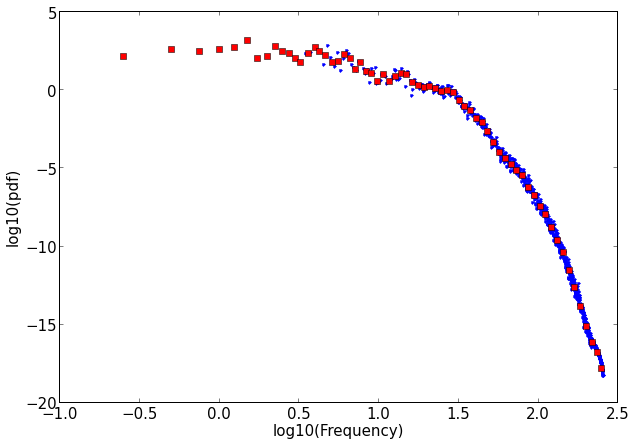
\includegraphics[width=5in]{Figures/binned_EEGpowerspectrum.png}
% \caption{Binned power spectrum}
% \label{binnedEEGpowerspec}
% \end{center}
% \end{figure}

%thomas notes: About here, a short pitch on pink noise is required to set the stage of the great method, and to justify the log log binning]}

Figure \ref{binnedEEGpowerspec} shows, in double logarithmic scale, the original 1024 bins (blue dots) of the pdf obtained from averaging the n power spectra of one sample, and the resulting ``compressed''  pdf with 100 log-bins. As we can see, the log-binning preserves the structure of the pdf.

In summary, we have built a probability density function of brain frequencies as captured by the Neurosky hardware, from the n power spectra of each sample. We have then used a log-binning method to reduce the 1024 bins from the original power spectrum to an arbitrary smaller number of log-bins (e.g., 100 log-bins on the Figure). This method makes a sort of statistical averaging by stacking, and then ``compresses" the result in way that it is easy to use in a classifier.

% {\bf NB:} I believe that the classifier does well because it can efficiently capture the overall level of activity for all log-bins, but also more local deviations. On the figure, we can see some local peaks mostly between $10^1$ and $10^1.5$, but in all other parts of the pdf though in a less visible way. I believe these deviations are quite unique and can make the difference in the classifier. We should indeed check this further if we want to understand to origins of the good results.

% {\bf Side note:} one way to investigate further would be to see indeed to what extent the ``compression", i.e. the small number of log-bins, affects the quality of the classifier. Another quite promising further research direction, would be to determine the minimum number of n power spectra, which should be taken into account to reach a target level of correct classification. This would be useful to determine what should be the most adequate sample size for a certain level of identification. This level might of course vary as a function of subjects and tasks.

%-----------


% \textcolor{red}{\bf [Maybe a schema would be great to help the reader get the point quickly]}

At this point, we have a one-dimensional signal flattened in the time dimension, computing the mean magnitude of each bin over all readings in the recording - a row vector with one entry for each each measured frequncy bin. 

\subsection{Classifier}

Support vector machines (SVM) are a set of supervised machine learning methods that take labeled example data to create a model that can be used to predict the classes of unlabeled data. SVMs use a hyperplane (an n-dimensional construct in n+1 dimensional space) to draw discriminatory boundaries between classes. In contrast to linear discriminant analysis, which has a long history of use in BCIs, SVMs select the hyperplane that maximizes distance from the nearest training points, which has been shown to increase the model's generalizability \cite{burges_tutorial_1998}.  For more on SVM's in BCI: \cite{garrett_comparison_2003,grierson_better_2011} 

In this study, we use LinearSVC, \cite{fan_liblinear:_2008} a wrapper for LibLinear exposed in Python through the ScikitLearn library. \cite{pedregosa_scikit-learn:_2011} We chose LinearSVC primarily because its underlying C implementation is very performant, and because linear kernels performed as well or better than nonlinear ones in early experimentation, corroborating the findings of previous studies. \cite{garrett_comparison_2003,lotte_review_2007}  We use the default settings for LinearSVC - a C of 1.0, squared hinge loss function, and a tolerance parameter of of 1e-4. 

% TODO:  explain what these parameters are, by e.g., providing the main formula of the LinearSVC.
% TODO: provide evidence for "as well or better than nonlinear ones"

\subsection{Per-user calibration}

We conducted a simulated calibration step for each participant. For each subject, we generated every possible pair of two tasks and cross-validated our SVM seven times on that subject's recordings for those two tasks. We used ScikitLearn's built-in cross-validation toolkit, which was configured to perform each of the seven cross-validation steps using different splits of trial data in the training and testing sets. For every task pair processed, we recorded mean classification across all cross-validation trials. We repeated this calibration process for all users at every combination of recording length and (log-)bin size. 

As an additional performance audit, we timed our SVM at training time and testing time. We fit an SVM to all the data for two task-pairs from two randomly-selected subjects, and repeated this process ten thousand times at different bin sizes and different lengths. We report the minimum time of each ten thousand attempts. In order to establish a proper estimate, we time the SVM after all data has been loaded to memory, disregarding the time it takes to load the data from disk.
\section{\uppercase{Results}}

\subsection{Experiment 1}

\begin{figure}[!h]
  \vspace{-0.2cm}
  \centering
   {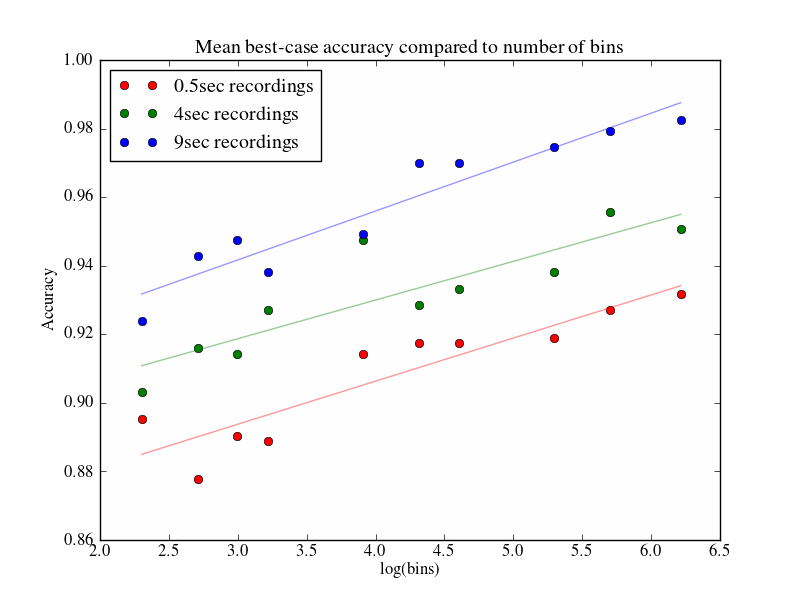
\epsfig{file = Figures/1-2.png, width = 5.5cm}}
  \caption{Mean best-case accuracy among all subjects compared to log of the number of bins in training data.}
  \label{fig:fig1}
  \vspace{-0.1cm}
 \end{figure}

Overall, both longer recording times and higher bin size are correlated with higher classifier accuracy. \textit{and what is important to report about this regression?}

\begin{figure}[!h]
  \vspace{-0.2cm}
  \centering
   {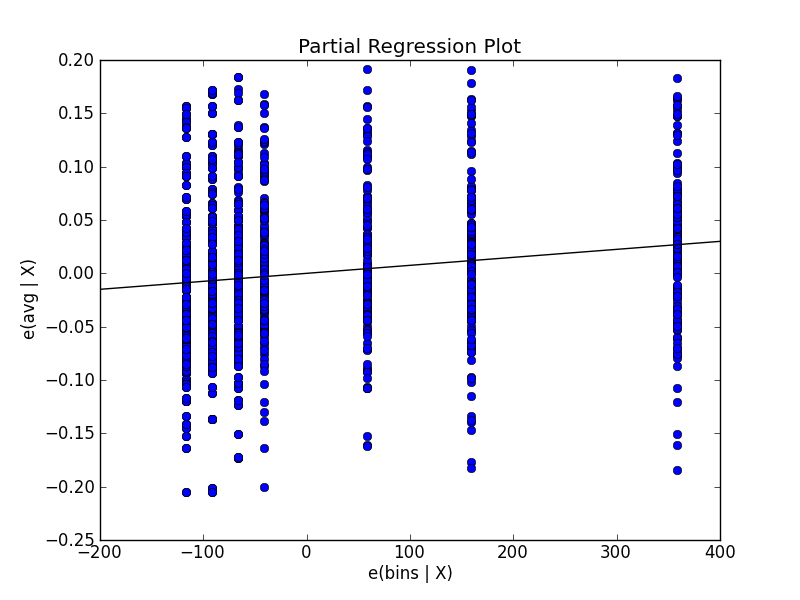
\epsfig{file = Figures/avg.png, width = 5.5cm}}
  \caption{SVM test time compared to number of bins in test set feature vector.}
  \label{fig:fig2}
  % \vspace{-0.1cm}
\end{figure}

\begin{figure}[!h]
  \vspace{-0.2cm}
  \centering
   {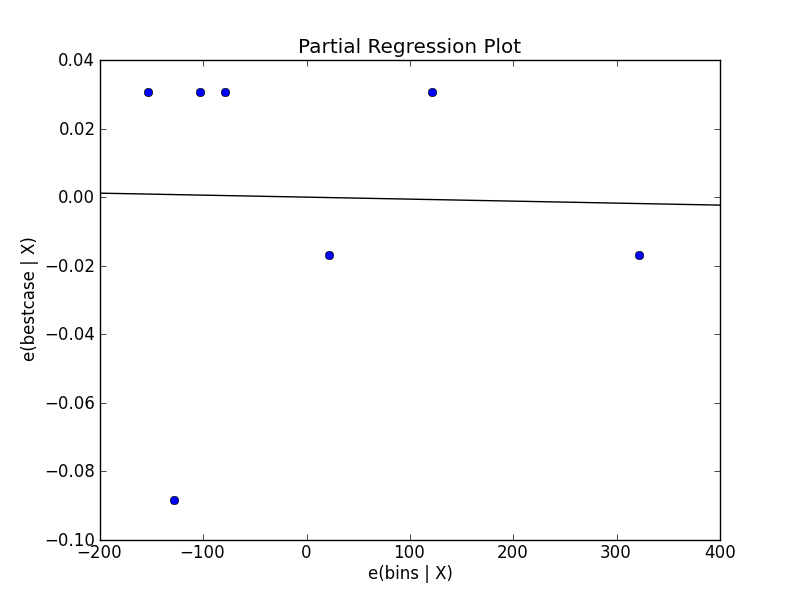
\epsfig{file = Figures/best.png, width = 5.5cm}}
  \caption{SVM train time compared to number of bins in training set feature vectors.}
  \label{fig:fig2}
  \vspace{-0.1cm}
\end{figure}


The number of bins is positively correlated with training and testing time. While test time grows linearly with the log of the number of bins. \textit{and what is important to report about this regression?}

\subsection{Experiment 2}

\begin{figure}[!h]
  \vspace{-0.2cm}
  \centering
   {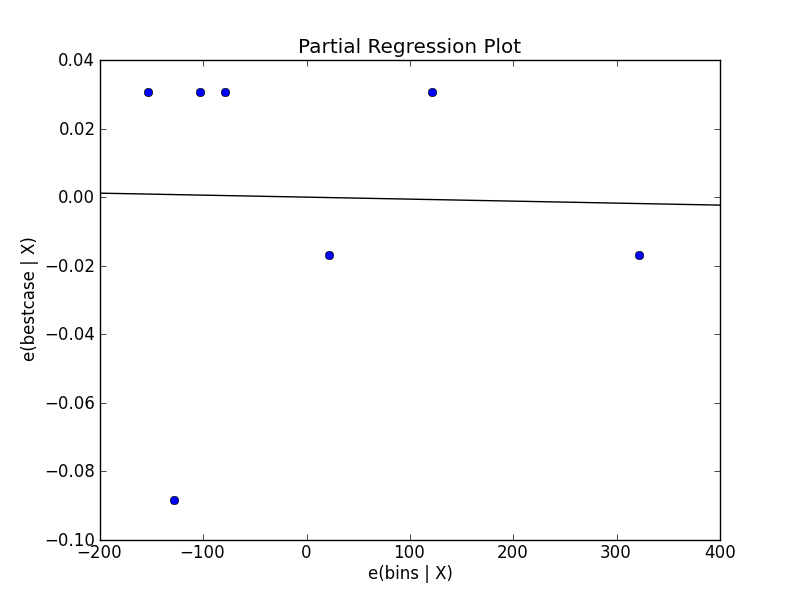
\epsfig{file = Figures/best.png, width = 5.5cm}}
  \caption{Mean best-case accuracy among all subjects compared to number of seconds of data in training set.}
  \label{fig:fig2}
  \vspace{-0.1cm}
\end{figure}

 The amount of data on which the classifier is trained is positively correlated with the classifier's accuracy on data from later recordings. \textit{and what is important to report about this regression?} The number of bins in training and testing data is also positively correlated with classifier accuracy.

\section{\uppercase{Discussion}}

\noindent We find that logarithmic binning dramatically decreases the computational expense of EEG-based calibration and classification without a significant detriment to accuracy. Further, we find that this technique is compatible with a training strategy capable of reaching acceptable classification rates with only thirty seconds of training data per mental task (compared to over two minutes with our baseline method). This strategy could enable speedy, per-user classification for commercial BCI systems.

The conclusions to be drawn from this study are limited in a few regards. First, calibration and classification were performed offline, so factors involving the user interface (such as feedback) are not taken into account. We cannot be sure, for instance, that our findings with short splices of ten-recordings data will persist when a system solicits recordings of only a second or under. Furthermore, a few of our tasks (e.g. the color task) relied on exogenous stimuli, which may be impractical in naturalistic settings for ergonomic reasons. Finally, we did not compare our findings to traditional signal processing methods in EEG.

Logarithmic binning could enable co-adaptive, online BCI with as few as one dry EEG sensor, making online calibration much more performant on mobile or embedded processors with limited computational resources. Alternatively, since logarithmic binning dramatically decreases the size of data fed to the classification algorithm, the technique could allow calibration to occur “in the cloud” - the BCI could pre-process the data on board, bin it, and ship this data to a more powerful server, which could process it online. By some combination of cloud-based and on-board processing, BCIs could gain from the accuracy of computationally expensive analytics without having to perform these computations on-board.

Future work could implement a system that calibrates a BCI online. Due to the small size of binned EEG signals, such a system could use a client/server architecture in which expensive processing (such as training multiple SVMs) is offloaded from the user’s system to a more powerful processor in teh cloud. This system could be used for the calibration of direct-control BCIs by attempting to find groups of tasks for which the classifier has high discriminatory power. A similar system could be used for long-term, affective recordings as well.

By collecting EEG data in the wild, we hope to discover more about how the mind behaves outside of laboratory environments. A particular interest is the non-stationary nature of neural recordings. By analyzing chronic EEG recordings at scale, we hope to make observations about how EEG signals change their expression over time, which could enable us to build more accurate BCIs that require less frequent re-calibration.

\vfill
\bibliographystyle{apalike}
{\small
\bibliography{references}}

\vfill
\end{document}

